\documentclass[11pt, a4paper]{article}
\usepackage[utf8]{inputenc}

\usepackage[margin=1in]{geometry} 
\usepackage{amsmath,amsthm,amssymb}
\usepackage[margin=1in]{geometry} 
\usepackage{amsmath,amsthm,amssymb}

\usepackage[slovene]{babel}
\usepackage{color}
\usepackage{graphicx}
\usepackage{amssymb}
\usepackage{amsmath}
\usepackage{mathtools}
\usepackage{commath}
\usepackage{ragged2e}
\usepackage[T1]{fontenc}
\usepackage[normalem]{ulem}
\usepackage{amsthm}
\usepackage{esvect}
\usepackage{float}
\usepackage{calrsfs}
\DeclareMathAlphabet{\pazocal}{OMS}{zplm}{m}{n}
\newcommand{\Ga}{\mathcal{G}}
\mathtoolsset{showonlyrefs} 

\newcommand\setItemnumber[1]{\setcounter{enumi}{\numexpr#1-1\relax}}


\newtheorem{theorem}{Trditev}[section]
\newtheorem{corollary}{Posledica}[section]
\newtheorem{lemma}[section]{Lema}
\theoremstyle{definition}
\newtheorem{definition}{Definicija}[section]
\theoremstyle{example}
\newtheorem{example}[section]{Primer}
\theoremstyle{izrek}
\newtheorem{izrek}[section]{Izrek}

\begin{document}
\begin{center}
\thispagestyle{empty}
\parskip=14pt%
\vspace*{3\parskip}%
\begin{Huge} Elektroopticni pojav \end{Huge}

By

Matic Tonin

ID No. (28181098)

Mentor 

(Rok Dolenec)

\rule{7cm}{0.4pt}

Pod okvirom:

FAKULTETE ZA FIZIKO IN MATEMATIKO, LJUBLJANA

9. 4. 2020

\end{center}
\pagebreak
\section{Naloga}
\begin{enumerate}
\item Izmerite kotno odvisnost prepustnosti polarizatorja za linearno polarizirano svetlobo.
\item Izmerite prepustnost dveh pravokotno postavljenih polarizatorjev, ko mednju postavite
še tretji polarizator in ga vrtite.
\item Dolocite Kerrovo konstanto PLZT keramike.
\item Analizirajte polarizacijo svetlobe po prehodu skozi dvolomno snov in dolocite debelino
tekocekristalne celice.
\end{enumerate}
\section{Postopek dela}
Nalogo smo razdelili na štiri dele in prav tako so bili postopki dela razdeljeni na štiri dele. 
\begin{enumerate}
\item Najprej smo morali izmeriti kotno odvisnost. Za začetek smo najprej postavili laser ter mikroampermeter tako, da  je laser zadel detektor na sredino. Zapisali smo zi začetni podatek o vrednosti toka na mikroampermetru, da smo vedeli, kolikšen je začetni svetlobni tok iz ozračja. Ugotoviti pa smo morali tudi, kako so polarizatorji orientirani. To smo storili tako, da smo pogledali, kako polarizator odbija svetlobo. \\
Zapisali smo si tudi kota, kjer je prepustnost minimalna in maksimalna in preverili, če sta 90° narazen. \\
Po korakih so nato vrteli polarizator in si zapisovali vrednosti toka, v odvisnotsi od zasuka, da bomo kasneje vedeli, kolikšna je moč prepuščene svetlobe pri izpisovanju na graf. 

\item Najprej smo nastavili polarizator, da je prepustnost minimalna. Nato smo postavili na klop še dodaten pilarizator in ga počasi vrteli po 5° in so v tabelo zapisovali vrednosti toka na mikroampermetru, da bomo kasneje vedeli, kolikšna je moč prepuščene svetlobe pri izpisovanju na graf. 

\item Najprej smo postavili vse aparature, kot nam kaže slika v navodilih za vajo. Torej: Fotodioda, polarizator, Kerrova celica, Laser. Paziti smo morali, da je vse nastavljeno tako, da laserski snop ne zadane elektrode na vzorcu in da svedloba pada na sredino fotodiode. Ko je vse postavljeno, vidimo, da je celica že brez el. polja dvolomna in to upoštevamo v naši formuli kot neko konstato premika. Nato začnemo meriti in si zapisujemo vse podatke v tabelo, da bomo kasneje narisali graf in iz fita funkcije odčitali Kerrovo konstanto B.

\item Pri tem delu vaje vzamemo vzorec, ki ima različne lomne količnike za različne orientacije. Za naš primer, imamo razliko v pravokotni in navpični smeri.
Najprej postavimo polarizator pod kotom 45° in celico, pravokotno na snop. Dobimo eliptično polariziranost. Za celico nato postavimo še drug polarizator, ki ga vrtimo in tako spreminjamo lege v elipsi. V smereh lastnih osi elipse ima prepuščena moč ekstrem in razmerje med max. in min. intenziteto je odvisno od fazne zakasnitve $\Delta \Phi =(k_{||} -k_{\perp})L$. Če je $\Delta \Phi=90°$, sta osi elipse enako dolgi in je izhodna polarizacija cirkularna. \\
V korakih po 10° vrtite analizator in si zapisujte vrednosti mikrometra. Zraven pa preverimo še smeri lastnih osi in eliptičnost prepuščene svetlobe. \\
Drugi del te vaje pa je namenjen meritvi debeline celice. Najprej postavimo vse aparature, kot piše v navodilih in pazimo na pravilno usmerjenost polarizatorjev. Nato s kotomerom merimo kot in na mikrometru moč prepuščene svetlobe, z intervali pod 5°. Nato doma narišemo krivuljo s pomočjo teorije, ki je podana v navodilih in jo bom navedel v samih postopkih dela. 
\end{enumerate}

\section{Meritve}
\subsection{Kotna odvisnost prepustnosti polarizatorja}

Svetlobni tok našega laserja smo merili z mikroamperom in  ugotovili, da ta v odvisnosti od časa rahlo niha. To nam dobro pokaže spodnji graf.
\begin{figure}[H]
	\centering
    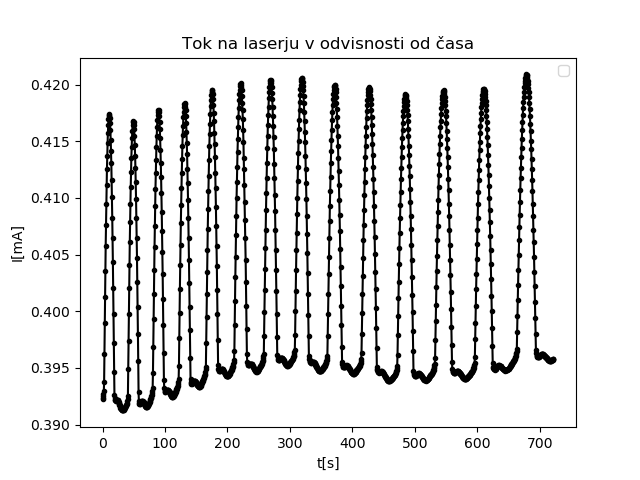
\includegraphics[width=12cm]{Tok_čas,dioda.png}
    \caption{Prikaz odvisnosti toka na laserju v odvisnosti od časa. Merili smo na intervalih 0.5 s}
\end{figure}

Vidimo, da tok niha glede na sredinsko vrednost z napao 5$\%$, zato lahko predpostavimo, da je konstanten. Če bi računali vrednost toka na laserju, bi ugotovili, da je: 


\begin{equation}
	\underline{I_0=0.402 \pm 0.15 mA} 
	\label{Povprečje toka na laserju}
\end{equation}

Ker sta si tok in moč sorazmerna, bo tudi izkoristek toka in moči med seboj sorazmeren. To bomo uporabili kasneje pri risanju grafa odvisnosti od toka. \\

Ko med naš laser in detektor postavimo še polarizator, se tok, ki ga zazna mikroampermeter spremeni v odvisnosti od tega, kako imamo polarizator obrnjen. To nam poda relacija: 

\begin{equation}
\label{Moč na diodi, en polarizator}
P_p=P_1\sin^2(\alpha + \delta )+P_0
\end{equation}

Kjer so $P_l, \delta, P_0$ prilagodljive konstante, ki nam jih izračuna naš fit grafa meritev premice.
Ker pa nimamo podane napetosti na našem detektorju, bomo to enačbo preprosto delili z začetno vrednostjo toka (\ref{Povprečje toka na laserju}) in tako dobili nekakšen graf izkoristka v odvisnosti od zasuka kondenzatorja.
Ko "pofitamo" funkcijo, dobimo:

\begin{figure}[H]
	\centering
    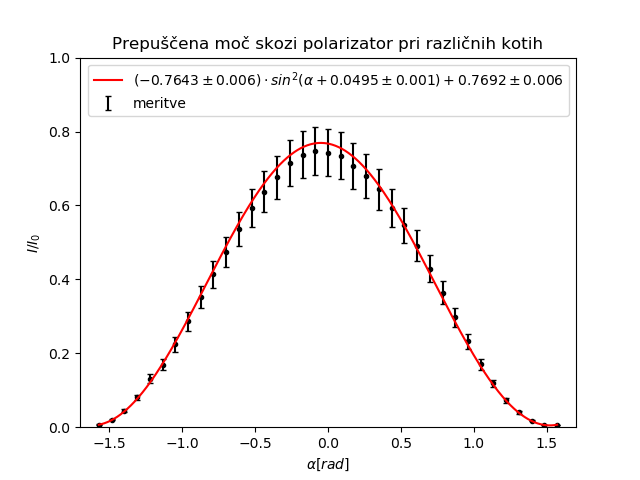
\includegraphics[width=12cm]{Izkoristek_kot,1_polarizator.png}
    \caption{Prikaz odvisnosti izkoristka na laserju v odvisnosti od zasuka polarizatorja}
\end{figure}

Kot lahko na grafu vidimo, je naš maksimum izkoristka doseže 77$\%$ toka na laserju. Malo pa nas zmoti to, da naša krivulja ni simetrična glede na kot $\alpha=0°$, ampak je majhno zamaknejna. Sklepamo, da se tu napaka pojavi zaradi majhne nenatančnosti pri pravokotnosti polarizatorja, ali pa, da orientacija polarizatorja ni dovolj precizno določena, kot je sam asistent navedel v podatkih.

\subsection{Prepustnost dveh pravokotno postavljenih polarizatorjev}

Postavimo polarizator iz prejšnjega dela tako, da je njegova prepustnost minimalna. Med njega in laser pa postavimo še en polarizator. 
Kot nam podajo navodila, je potem moč ali tok, ki jo zazna mikroampermeter enaka

\begin{equation}
\label{Moč na detektorju, dva polarizatorja}
P_p=P_1 \sin^2(2\beta + \delta) + P_0 
\end{equation}

kjer so $P_1, \delta, P_0 $ ponovno neke konstante, ki nam jih določi fit grafa funkcije. 
Princip za risanje grafa funkcije se ne bo spremenil, torej bmo ponovno izrisavali na graf nek izkoristek v odvisnosti od toka. Sledi, da je: 

\begin{figure}[H]
	\centering
    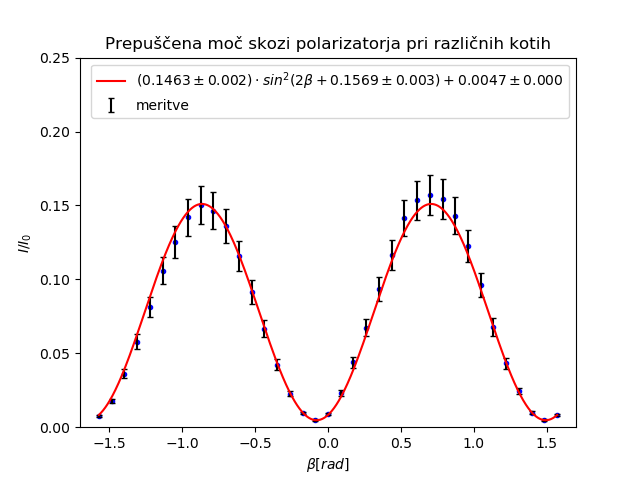
\includegraphics[width=12cm]{Izkoristek_kot,2_polarizator.png}
    \caption{Prikaz odvisnosti izkoristka na laserju v odvisnosti od zasuka polarizatorja}
\end{figure}

Ponovno vidimo, da je naš graf rahlo zamaknjen glede na simetrično os $\beta=0°$, zato nam to potrjuje, da je napaka sistemska, torej da naš sistem ni bil pravilno nastavljen. Torej, ali da polarizator ni bil pravilno poravnan, ali pa da ima že sam polarizator vgrajeno napako za nek kot $\delta \beta$. To bomo na koncu vaje lahko primerjali. 
Za samo prepustnost moči pa vidimo, da se je maksimum prepustne moči zmanjšal na 15\%. Vidimo pa tudi, da se pojavita dva polarizatorska vrhova namesto enega. Tako smo sedaj dobili maksimume toka pri $\frac{\pi}{4}$ in $-\frac{\pi}{4}$ ( če seveda ne upoštevamo zamika.

\subsection{Meritev Kerrove konstante PLZT keramike}
Najprej postavimo vse aparature, kot je napisano v postopku dela, nato pa začnemo meriti napetost na celici s tem, da moramo upoštevati relacijo, da je napetost na merilnem izhodu 1/1000 tiste, ki je na Kerrovi celici. Meritev izvajamo hitro, da se nam $\Phi_0$ (ta številka je posledica nehomogenega osvetljevanja keramike na celici. Glavni vzrok je v tem, da ker keramika nekoliko absorbira svetlobo, že v njej pride do notranjega fotoefekta in tako se nosilci naboja lahko gibljejo prosto v zunanjem el. polju. Tako, z izvajanjem hitrejše meritve, zmanjšamo čas absorbcije svetlobe in s tem zmanjšamo spreminjajnje vrednosti te "konstante").
Ko namerimo vse vrednosti toka na laserju in napetosti na Kerrovi celici, se lotimo risanja grafa. 

Za našo PLZT keramiko pa imamo dve določeni konstanti in sicer:

\begin{equation}
\label{Razmik in debelina med ploskvama}
d=1.4 mm \quad L=1.5 mm
\end{equation}

Vemo pa tudi, da je moč na celici odvisna z relacijo. 

\begin{equation}
P_{p}=P_{1} \sin ^{2}\left(\pi B L U^{2} / d^{2}+\Phi_{0} / 2\right)
\label{Kerrova konstanta}
\end{equation}
Kjer so $P_1, B, \Phi_{0}$ neki parametri, ki jih bomo določili iz fitanja grafa na našo krivuljo.

Po pofitamo graf, dobimo krivuljo: 
\begin{figure}[H]
	\centering
    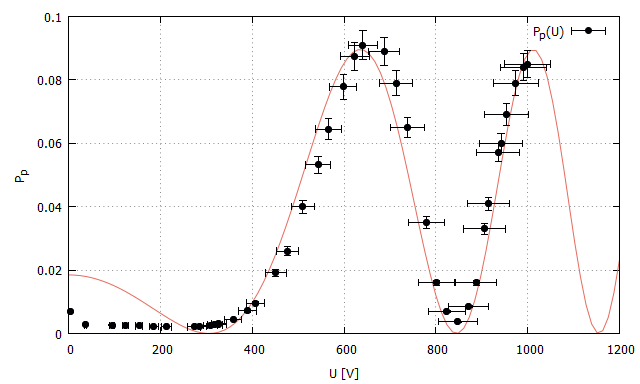
\includegraphics[width=12cm]{Izkoristek_kot,Kerrova celica.png}
    \caption{Prikaz spremembe toka na Kerrovi celici v odvisnosti od kota}
    

\end{figure}
Ta graf je malo drugačen od drugih, saj sem uporabil namesto programa python, program Gnuplot, ki je hitreje in lepše izrisal in prilagodil graf našim konstantam. 
Tako dobimo parametre: 
$$P_1= 0.0900 \pm 0.002625 \quad(2.929\%) $$ 
$$ B=2.11 \cdot 10^{-9} \pm 2.698 \cdot 10^{-11} \frac{m}{V^2} \quad (1.282\%)$$
$$\Phi_0= -0.94 \pm 0.07124 \quad (7.557\%)$$
\pagebreak
\subsection{Polarizacija svetlobe pri prehodu skozi dvolomno snov}
\subsubsection{Prikaz eliptične slike, ki jo nariše vektor $\vec{E}$}
Pri tej meritvi imamo dvolomni material z dvema različnima lomnima količnikoma v eno in drugo smer: 
\begin{equation}
\label{Lomni količniki}
n_{||}-n_{\perp}=0.174
\end{equation}

Po vsej postavitvi naših aparatur, bi morali z meritvami zaznati eliptično polarizacijo.
Če najprej narišemo zgolj odvisnost toka od našega zasuka, dobimo graf:

\begin{figure}[H]
	\centering
    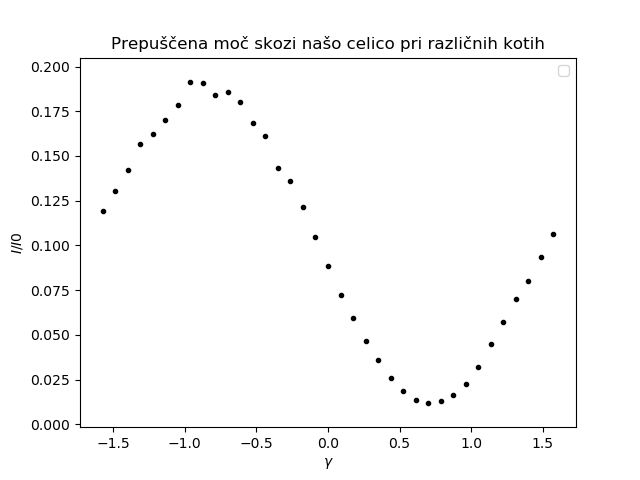
\includegraphics[width=12cm]{Izkoristek_kot,elipsa.png}
    \caption{Slika projekcij na x in y os in prikaz eliptične polarizacije}
\end{figure}

 To lahko preverimo z risanjem našit točk na graf. Risali pa bomo projekcije razmerja začetne in končne moči na x in y os, v odvisnosti od kota $\theta$. 
Torej dobimo graf:

\begin{figure}[H]
	\centering
    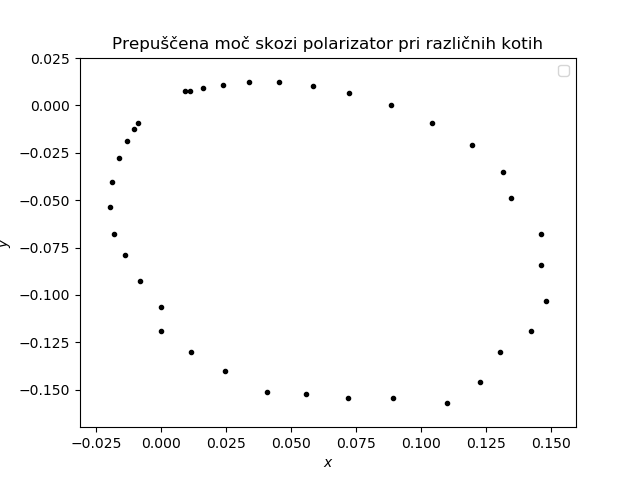
\includegraphics[width=10cm]{Elipsa.png}
    \caption{Slika projekcij na x in y os in prikaz eliptične polarizacije}
\end{figure}

Kakor vidimo, ne dobimo popolne slike elipse. Najbolj očitno se to vidi pri prehodu iz pozitivnoh x na negativne x, torej ko sinus spremeni svoj predznak zaradi kota. Sklepamo, da je glavni faktor tega nenatančnost polarizatorja, ki se je nam je dajala določene fazne zamike že pri prejšnjih delih naloge in nam je tu rahlo pokvarila obliko elipse. Hkrati pa je verjetno napaka tudi v tem, da so bile mogoče kakšne meritve nenatančne, kar sklepamo iz točke T(0.145,-0.084), ki najbolj iztopa iz eliptične slike na desni polosi. Ta tokča je na Sliki 5 prikazana kot vrh prvega grafa sinusne funkcije in vidimo, da je ta vrh precej raztresen in zato so tudi točke ob polosi elipse raztresene.  \\
\subsubsection{Meritev razdalje med ploskvama}
Za drugi del pa potrebujemo izračunati, kolikšna je debelina naše celice.
To laho izračunamo, če merimo kot odbitega snopa in nato narišemo vrednosti izkoristka svetlobe v odvisnotsi od kota. Če na naše točke nato nanesemo fit: 
$$P_{p}=P_{1} \sin ^{2}(\Delta \Phi / 2)+P_{0}$$
 kjer so $P_1, P_0$, konstante, v vrednosti $\Delta \Phi$ pa se skriva kot in sicer:
 
$$\Delta \Phi=k_{\|} L_{1}-k_{\perp} L_{2}-k_{0} L_{3}=\frac{2 \pi d}{\lambda}[\sqrt{n_{\perp}^{2}-\sin ^{2} \alpha}-\sqrt{n_{\|}^{2}-\sin ^{2} \alpha}]$$

Lahko iz tega dobimo našo vrednost d, ki nas zanima. Poglejmo si najprej sliko grafa: 
\begin{figure}[H]
	\centering
    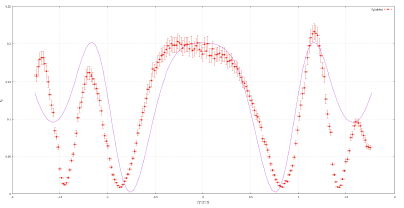
\includegraphics[width=15cm]{Debelina.png}
    \caption{Prikaz odvisnosti izkoristka od kota s fitano funkcijo}
    
Naš fit pa nam nato poda, da je debelina našega vzorca 
$$\underline{d=15.6 \mu m}$$

Vidimo, da naš fit, zaradi zahtevnosti meritve precej odstopa od naših izmerjenih meritev. Zato sklepamo, da je napaka meritve konstante debeline velika, vsaj 20 \%.

Prav tako je bil zadnji graf narisan v Gnuplotu, saj na žalost nisem znal risati s pythonom.
\end{figure}
\end{document}